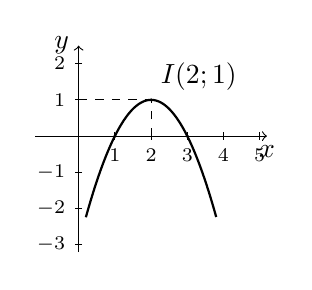
\begin{tikzpicture}[scale=0.46]
    \draw[->] (-1.2,0) -- (5.2,0) node[below] {$x$};
    \draw[->] (0,-3.2) -- (0,2.5) node[left] {$y$};

    \foreach \x in {1,2,3,4,5}
        \draw (\x,0.1) -- (\x,-0.1) node[below] {\scriptsize $\x$};

    \foreach \y in {-3,-2,-1,1,2}
        \draw (0.1,\y) -- (-0.1,\y) node[left] {\scriptsize $\y$};

    \draw[smooth, samples=200, domain=0.2:3.8, thick]
        plot (\x, {-\x*\x + 4*\x - 3});

    \fill (1,0) circle (1.3pt);
    \fill (3,0) circle (1.3pt);
    \fill (2,1) circle (1.3pt);
    \draw[dashed] (2,0) -- (2,1);
    \draw[dashed] (0,1) -- (2,1);
    \node[above right] at (2,1) {$I(2;1)$};
\end{tikzpicture}
